\documentclass[main.tex]{subfiles}
\pagestyle{main}%%%
\begin{document}

\chapter{Préservation de l'invariance par rotation sur maillage cartésien}
\vspace{-13mm}
\begin{flushright}
{ \Large\sf ou Vous avez dit trèfle à 4 feuilles ?\ }
\end{flushright}
%\mylettrine{C}{e} chapitre aurait pu ce nommer \og Vous avez dit trèfle à 4 feuilles ? \fg{}, car oui en effet, comme nous allons le voir au début de ce chapitre, discrétiser notre modèle avec des schémas standards va produire une 
%
%\mylettrine{T}{ransporter} (ou diffuser) une quantité invariante par rotation n'est pas chose facile. Pour illustrer cela, nous allons montrer dans un premier temps les résultats obtenus, lorsqu'on discrétise le modèle présenté au chapitre précédent avec des schémas classiques.  Nous examinerons ensuite les diverses sources causant

\mylettrine{C}{onsidérons} le modèle que nous avons construit au chapitre précédent avec pour donnée initiale des densités invariantes par rotation. Le champ de vitesse (donnée par ces mêmes densités) est donc invariante par rotation. Ainsi pour tout temps nos densités devraient être invariante par rotation. Sauf qu'avec les schémas numériques classiques, cette propriété n'est pas du tout conservée au fil du temps... Comme nous allons le présenter au début de ce chapitre, les lignes de niveaux, au départ circulaires, vont peu à peu se déformer devenant progressivement carrées puis prenant plus tard la forme d'un trèfle à 4 feuilles !... Deux pistes seront alors étudiées~:
\begin{myitemize}
\item défaut du schéma de diffusion
\item défaut du schéma de transport
\end{myitemize}


\noindent Un correctif sera finalement proposé. 

\section{Présentation du problème}
Sans plus tardez, présentons le problème en image. Sur la Figure~\ref{fig:trefle}, est présenté une simulation numérique du modèle EDP construit au chapitre précédent avec~:
\begin{myitemize}
\item un schéma à 5 points classique pour la diffusion,
\item un WENO5 (avec splitting directionnel) pour le transport.
\end{myitemize}
\begin{figure}
\centering
HEP FIGURE
\caption{\label{fig:trefle} Simulations numériques réalisées avec un WENO5 pour le transport et un Laplacien classique à 5 points pour la diffusion. Numerical simulations with the standard WENO5 stencil for the
specific set of parameters. Partant d'une donnée initiale circulaire, 
une structure en forme de trèfle apparaît.}
\end{figure}
La forme en forme de trèfle apparaît ici clairement. 

\section{Le schéma de diffusion}
\subsection{Influence de la condition limite}
Le schéma associé à la diffusion a été le premier à être incriminé. En effet dans l'équation~REFF ??\todo{eqref}, la condition limite (CL) est imposée au bord du domaine de calcul $\Omega$, domaine qui est carré. La CL ne vérifie donc pas, dès le départ, l'invariance par rotation. Ceci est illustré sur la Figure~\ref{fig:ligne_nvx_laplace_carre} qui présente la solution de l'équation
\begin{equation}\label{eq:pression_iter1}
\left\{
\begin{aligned}
-\Delta \Pi(\vecx) &= P(t=0,x) & \quad \textrm{ dans }  \Omega , \\
\Pi(\vecx) &=0 & \quad \textrm{ sur  } \partial \Omega,
\end{aligned}
\right.
\end{equation}
qui n'est autre que l'équation résolue à la première itération ($M$ étant initialisé au dessus du seuil d'hypoxie, on a alors au départ $\gammapp=1$ dans l'équation REF. De plus, comme $N=0$ au départ, on obtiens alors $\dive \vit = P$, car $k\equiv1$). Dans les itérations suivantes certes le second membres de l'équation va varier, mais cela ne va pas changer le fait que la forme du bord impacte sur les lignes de niveaux.
\begin{figure}
\centering
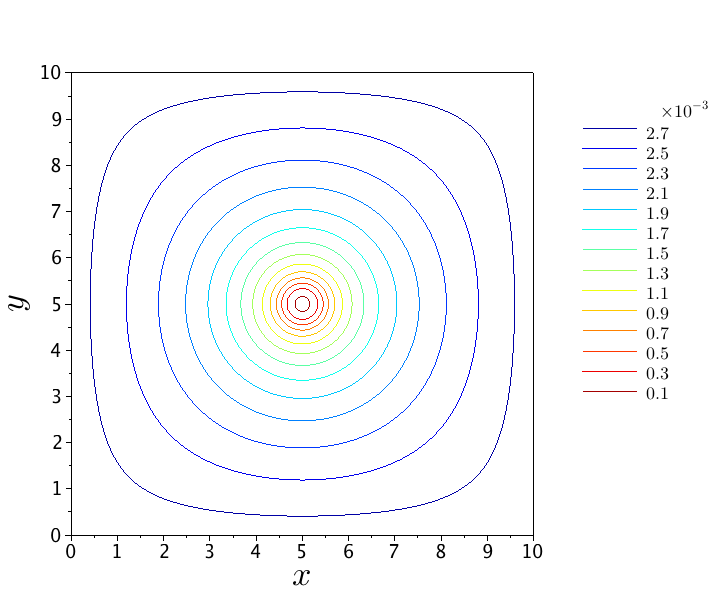
\includegraphics[width=.7\textwidth]{simu/trefle_track/point3_0/track_10x10_7/pression_2.png}
\vspace{-4mm}\\
\caption{\label{fig:ligne_nvx_laplace_carre} Résolution de la pression donnée par un laplacien. La forme du domaine de calcul carré impacte sur le résultat.}
\end{figure}

L'effet carré sur les lignes de niveaux de la pression, apparait surtout près du bord du domaine de calcul. Ainsi, pour tenter de palier à ce défaut, la première idée fut de considérer un domaine plus grand, laissant une sorte de couche limite pour absorber les déformations. Des simulations numériques de notre modèle ont été réalisées en doublant la longueur dans chaque direction (la taille d'une maille restant inchangée, on double aussi le nombre de maille). Malheureusement, une forme de trèfle est toujours visible. On a même du mal à distinguer visuellement si il y a eu une amélioration. Visiblement cette couche limite ne suffit pas. Imposons donc la CL sur un cercle, de sorte à ce que celle-ci soit invariante par rotation. Considérons alors un disque $\mathcal{D}$ inclus dans notre domaine de calcul initial $\Omega$ et imposons la CL de dirichlet sur son bord. L'équation~REFF\todo{eqref} devient alors~: 
\begin{equation}\label{eq:pression_iter1_mask}
\left\{
\begin{aligned}
-\Delta \Pi(t,\vecx) &= F(t,\vecx) & \quad \textrm{ dans }  \Omega , \\
\Pi(t,\vecx) &=0 & \quad \textrm{ sur  } \partial\mathcal{D},
\end{aligned}
\right. \quad \forall t>0
\end{equation}
Pour résoudre cela on procède par pénalisation de tout ce qui est à l'extérieur du disque~:
\begin{equation}
- \Delta \Pi(t,\vecx) = F(t,\vecx) + \frac{1}{\epsilon} \Pi \mathds{1}_{\mathcal{D}^c}(\vecx),
\end{equation}
où $\mathcal{D}^c$ désigne le complémentaire de $\mathcal{D}$. Cette technique nous garantit ainsi l'invariance par rotation de $\Pi$ si $F$ l'est, comme on peut le voir sur la Figure~REF. Les simulations numériques réalisées avec ce masque circulaire ne montre qu'une très légère amélioration \todo{Montrer graphique?} de la forme~: le trèfle persiste. 
Explorons alors une autre piste. 

\subsection{Schéma à 9 points}
La forme du trèfle fait très clairement apparaître les directions du maillage. Il est alors légitime de se demander si un schéma avec un stencil à 9 points ferait aussi apparaître ce genre de forme. 
\begin{figure}[h]
\subfloat[\label{fig:schema_laplace_9pts_classique}Schéma classique]{
\resizebox{.49\textwidth}{!}{\setlength{\unitlength}{0.01\textwidth}
\begin{picture}(110,105)
%%\rect{0}{0}{110}{105}

\Huge
\squaremesh{10}{40}{2}
\multiput(10, 10)(0, 40){3}{\multiput(0, 0)(40, 0){3}{\circle*{5}}}

\put(12,3){%%% calque des legendes de noeuds
\multiput(0, 0)(0, 80){2}{\multiput(0, 0)(80, 0){2}{$-1$}}
\multiput(40, 0)(0, 80){2}{$-4$}
\multiput(0, 40)(80,0){2}{$-4$}
\put(40,40){$20$}
}
\put(85,95){\scalebox{2}{$\times \sfrac{1}{6h^2}$}}

\end{picture}
}}
\subfloat[\label{fig:schema_laplace_9pts_custom}Autre schéma découlant d'une méthode mixte VF/EF présentée dans l'annexe annexe~\ref{chap:anx_methode_mixte_VFEF}]{
\resizebox{.49\textwidth}{!}{\setlength{\unitlength}{0.01\textwidth}
\begin{picture}(110,105)
%%\rect{0}{0}{110}{105}

\Huge
\squaremesh{10}{40}{2}
\multiput(10, 10)(0, 40){3}{\multiput(0, 0)(40, 0){3}{\circle*{5}}}

\put(12,3){%%% calque des legendes de noeuds
\multiput(0, 0)(0, 80){2}{\multiput(0, 0)(80, 0){2}{$-1$}}
\multiput(40, 0)(0, 80){2}{$-2$}
\multiput(0, 40)(80,0){2}{$-2$}
\put(40,40){$12$}
}
\put(85,95){\scalebox{2}{$\times \sfrac{1}{4h^2}$}}

\end{picture}
}}
\caption{\label{fig:schema_laplacien}Poids associés à chacun des points du stencil à 9 points de schémas discrétisant le laplacien ($h$ étant le pas d'espace, égal dans chaque direction).}
\end{figure}
Le premier schéma à 9 points essayer est le schéma classique, présenté notamment ???\todo{bib ref}, ayant des poids comme indiqué sur la Figure~\ref{fig:schema_laplace_9pts_classique}. Aucune amélioration n'a malheureusement été constatée ... Un second schéma à 9 points a été imaginé à partir d'une méthode mixte éléments finis/volumes finis.
%%%% Figure basculées en annexe
Sur chaque maille $\mathcal{M}$, une approximation par un polynôme $\mathbb{Q}_1$ est réalisée à partir des valeurs aux quatre coins de la maille. Le flux au travers du volume de contrôle est alors calculé comme l'intégrale sur le bord de ce volume, de la dérivée du polynôme. Les détails concernant cette méthode sont présenté en  annexe~\ref{chap:anx_methode_mixte_VFEF}. Il y est notamment montré que ce schéma mixte se ramène en réalité à un schéma à 9 points avec des poids un peu différents, comme présenté dans la Figure~\ref{fig:schema_laplace_9pts_custom}. 
Ici encore le trèfle persiste. Explorons alors une autre piste.

\section{Le schéma de transport}
Afin de démontrer que le responsable du trèfle est le schéma de transport, travaillons sur un modèle plus simple, le plus simple possible. Il sera à priori incapable de reproduire la biologie que l'on souhaite décrire mais il aura l'avantage de toujours présenter cette forme en trèfle. 
Ce nouveau modèle est construit à partir du modèle complet présenté au chapitre précédent, en faisant les simplifications suivantes~:
\begin{myitemize}
\item On enlève les parties modélisant les traitements cliniques. On peut donc ainsi considérer une seule et unique population proliférante.
\item On supprime la partie vascularisation. Les taux de croissance $\gammapp$ et $\gammapd$ sont alors considéré constant, égaux à~1.
\item On supprime le compartiment nécrosé, quitte à considérer que celle-ci est instantanément éliminée.
\end{myitemize}
Le modèle complet en est alors réduit à~:
\begin{equation}
\left\{ \begin{aligned}
\partial_t P + \dive (\vit P) &= 0 \\
\dive \vit &= P  \\
\vit &= \nabla \Pi
\end{aligned} \right.
\end{equation}
Notez qu'en injectant la seconde égalité dans la première équation, on obtient~:
\begin{equation}
\partial_t P + \vit \nabla P = -P^2
\end{equation}
Pour pouvoir incriminer le schéma de transport
\end{document}